\documentclass{article}

\usepackage{graphicx}

\title{SmartCity used by Paris, London, New York and Tokyo!}

\begin{document}
\maketitle
\section{Introduction}

Pour ce projet, nous avons décidé de réaliser un DSL graphique. En effet, il semble raisonnable de penser que certains utilisateurs potentiels ne soient pas familiers avec la programmation. Or un DSL graphique semble être une bonne manière de créer un cadre de simulation d'une SmartCity (ou d'un SmartCampus) de manière accessible à un large public en restant le plus expressif possible. Notre interface permet de facilement créer des sensors, de leurs associer une loi, et de simuler le sensor sur une période de temps que l'utilisateur peut préciser. Nous avons choisi l'extension ``E4: Real Time Simulations''.

\begin{figure}
  \centering
  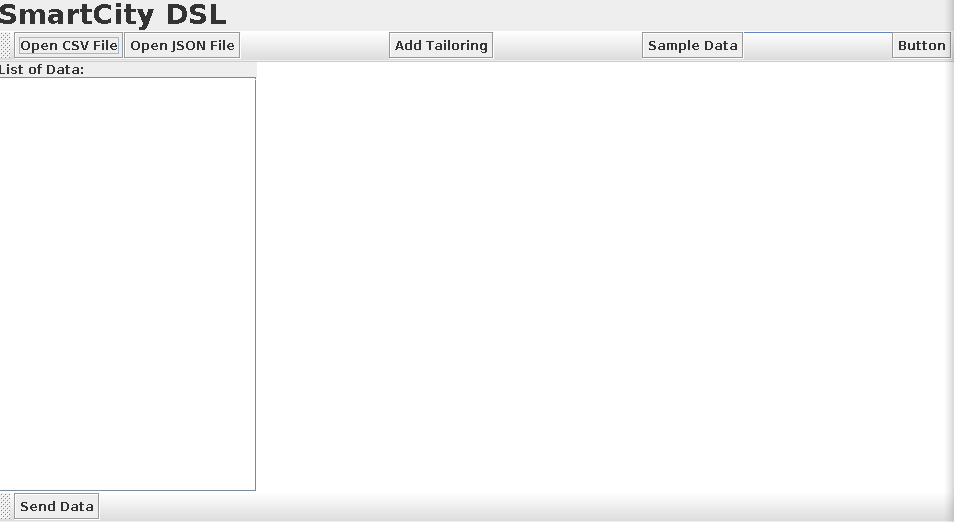
\includegraphics[width=8cm]{Figs/intro.png}
  \caption{The main window of our graphical DSL}
  \label{fig:intro}
\end{figure}



\end{document}
